\documentclass[a4paper,11pt,openright]{report}
\setlength{\parindent}{0pt} % set noindent for entire file

\usepackage[utf8]{inputenc}
\usepackage[a4paper,top=25mm,bottom=25mm,left=15mm,right=20mm]{geometry}
\usepackage{xcolor,graphicx}
\usepackage{amsmath}
\usepackage{setspace}
\usepackage{sectsty}
\usepackage{etoolbox}
\usepackage{enumitem}
\usepackage{listings}
\usepackage{textcmds}
\usepackage{times}

\graphicspath{ {/home/saran/Analytics/Jun_30/} }

\lstdefinestyle{mystyle}{
	backgroundcolor=\color{white},
	basicstyle=\ttfamily\footnotesize,
	breakatwhitespace=false,
	breaklines=true,
	captionpos=b,
	keepspaces=true,
	showspaces=false,
	showstringspaces=false,
	showtabs=false,
	tabsize=4
}

\lstset{style=mystyle}

\begin{document}
\singlespacing
\pagestyle{plain}

\begin{small}
\begin{center}
\textbf{Assignment: Inner/Left/Right/Cross Join Operations} \\
Date: 29/09/2020 \hspace{2mm} Name: D.Saravanan
\end{center}
\end{small}

\vspace{10px}

\begin{footnotesize}
1. Create two tables (with more than two columns), perform all the join operations
and display the output.
\end{footnotesize}

%figure_1
\begin{figure}[ht!]
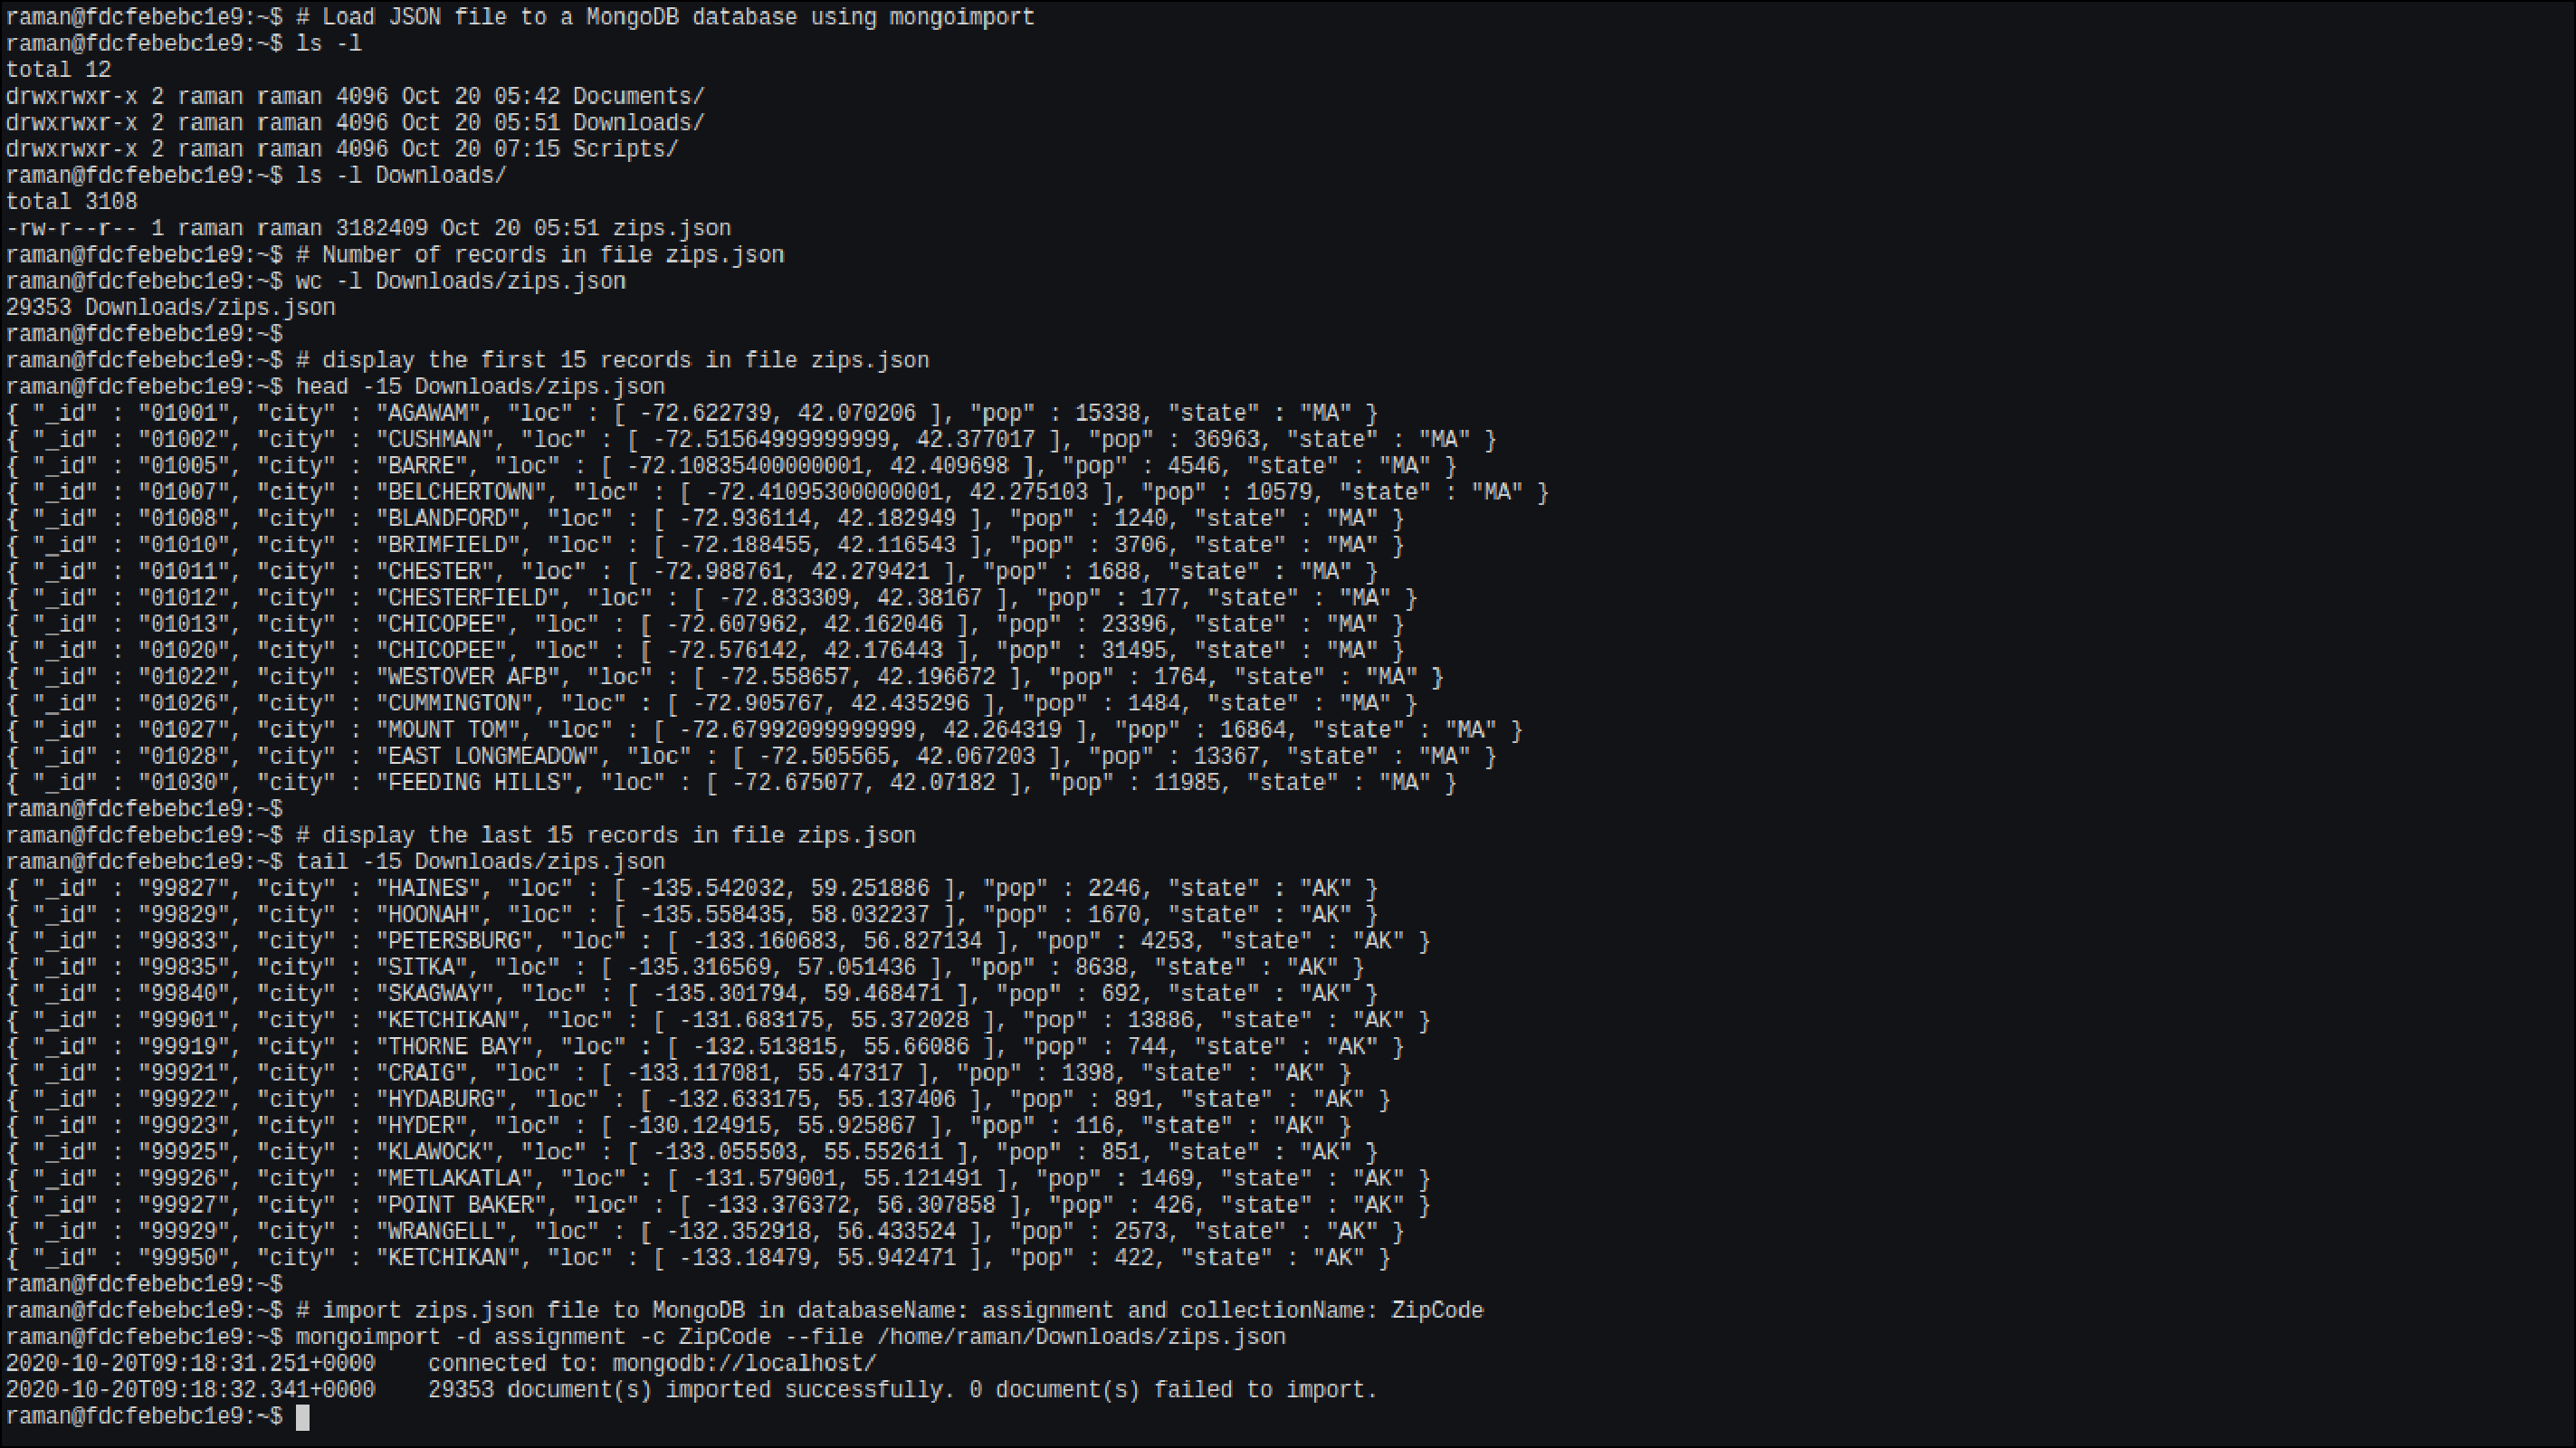
\includegraphics[width=20cm,height=10cm,keepaspectratio]{image1.pdf}
\centering
\end{figure}

\vspace{20px}

%figure_2
\begin{figure}[ht!]
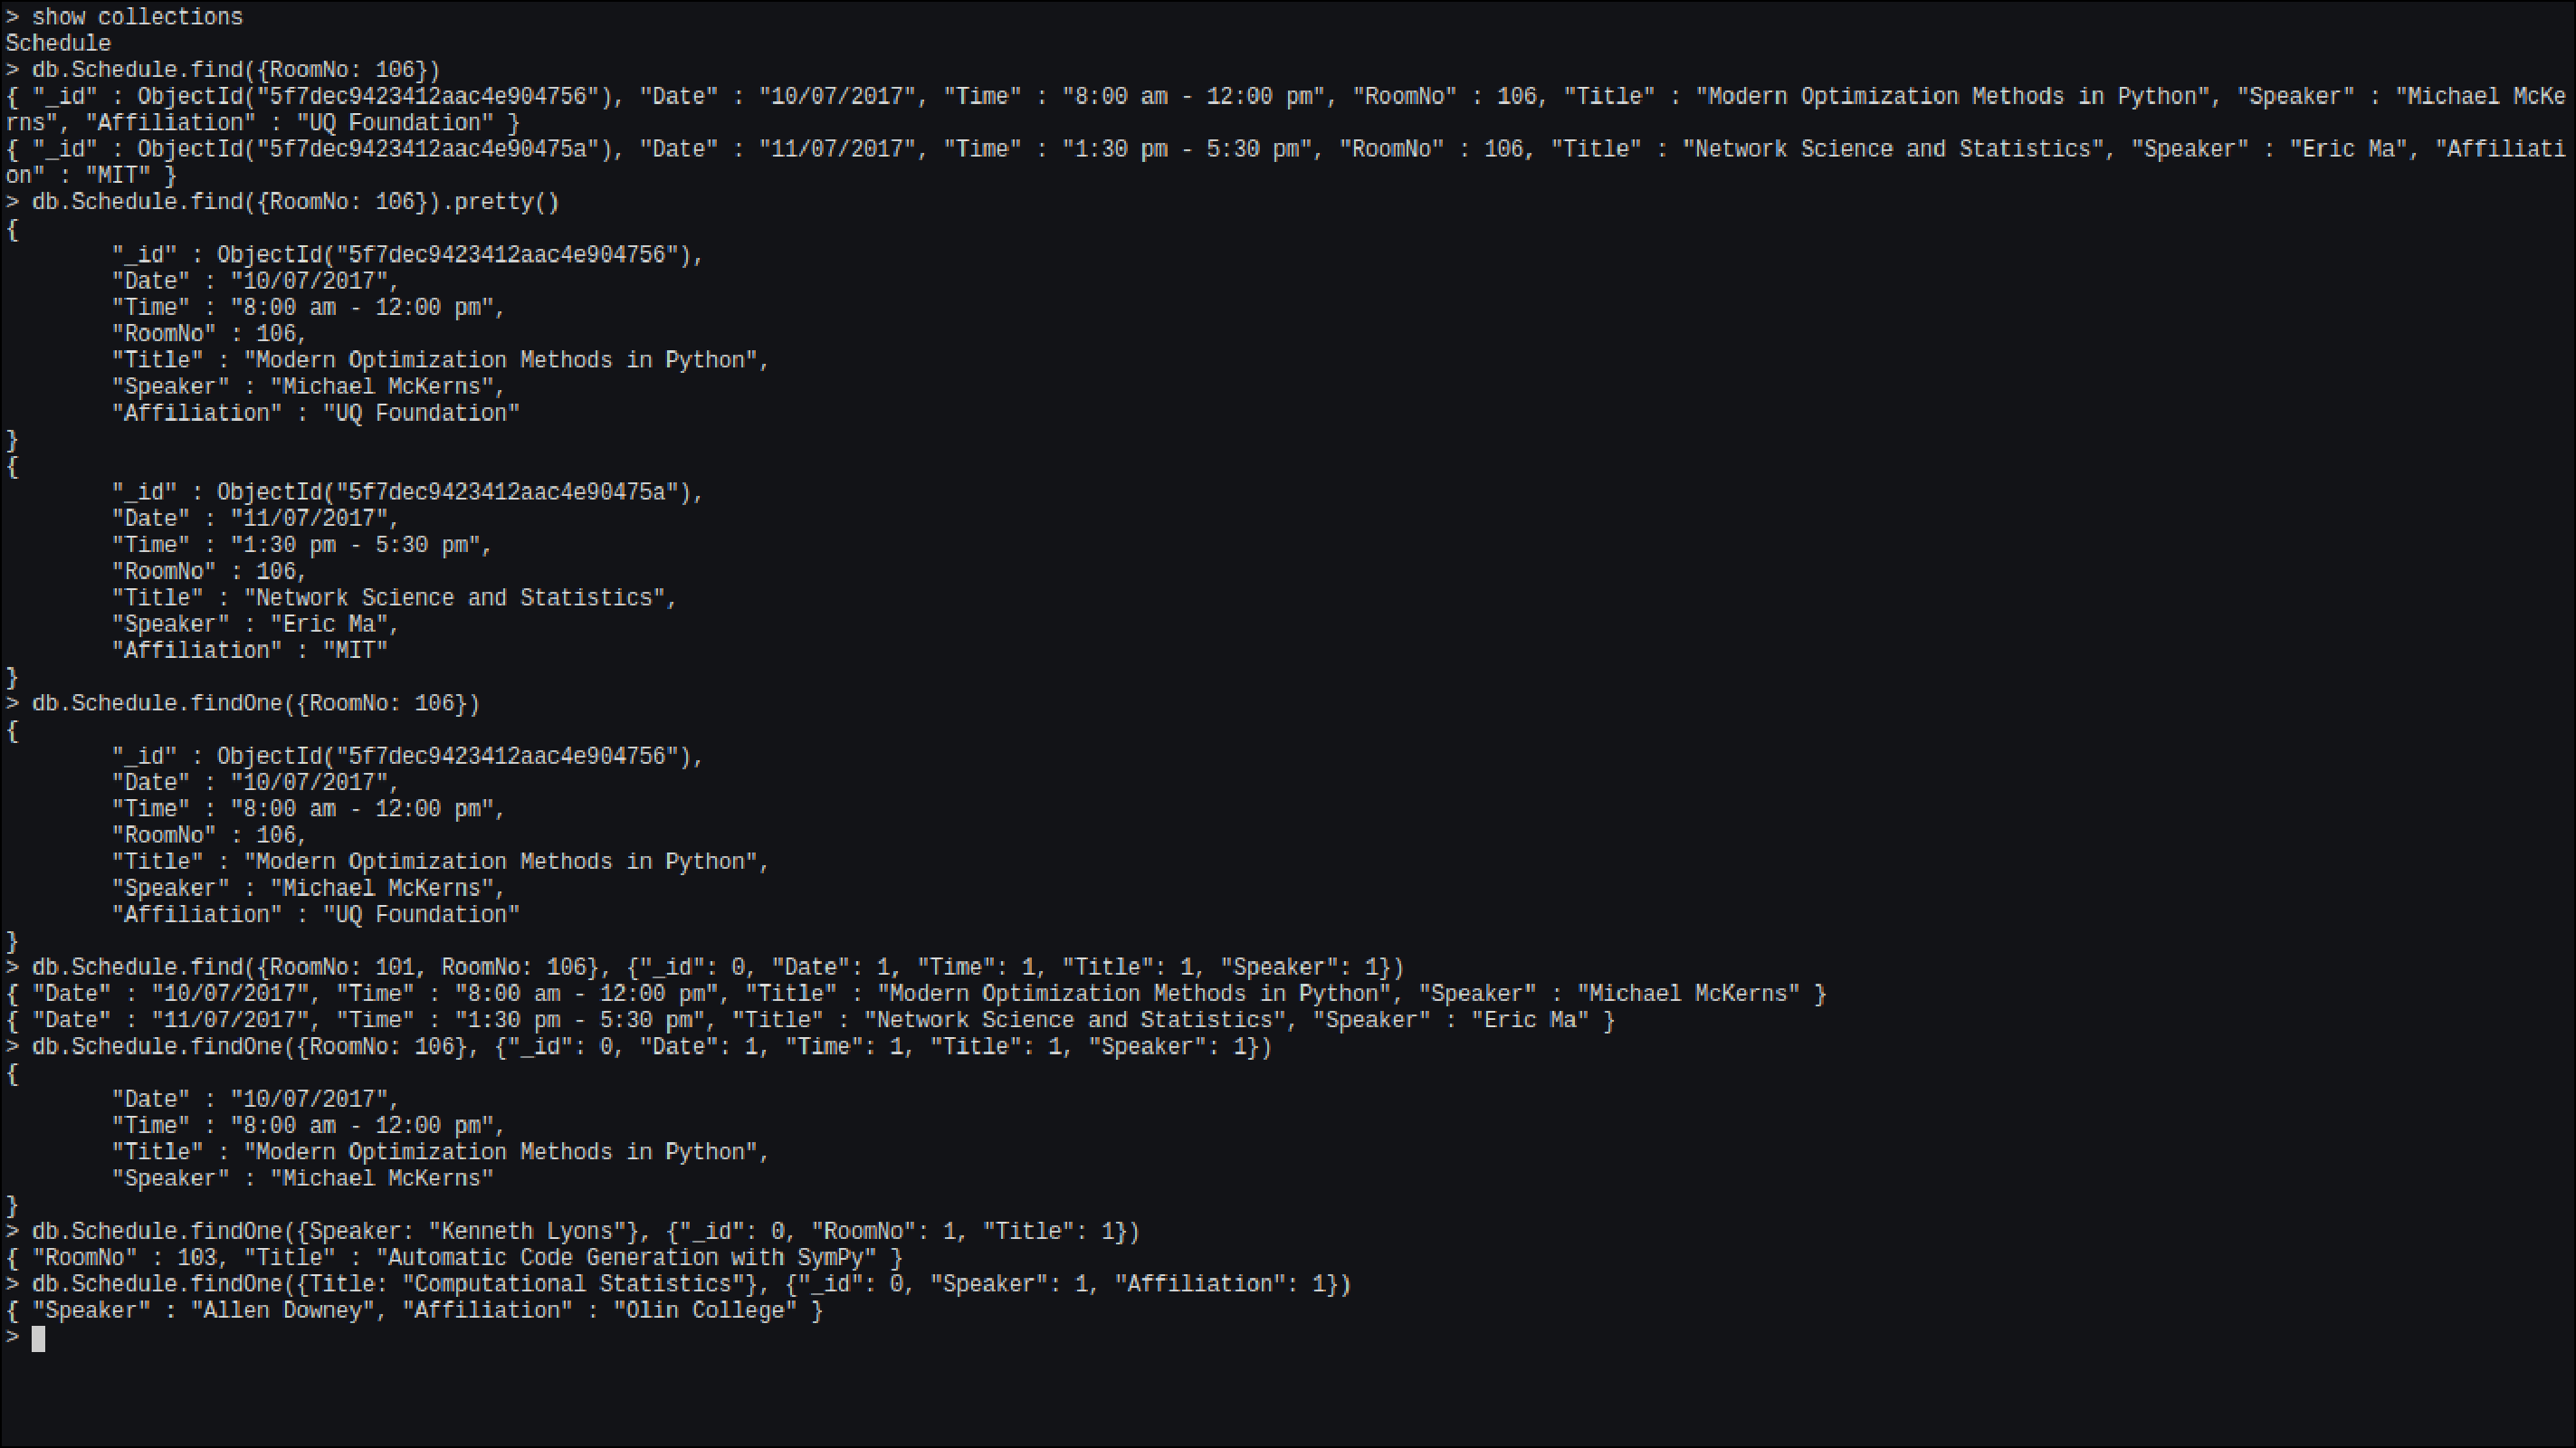
\includegraphics[width=20cm,height=10cm,keepaspectratio]{image2.pdf}
\centering
\end{figure}

\pagebreak

\vspace{10px}

{\footnotesize Inner Join}

%figure_3
\begin{figure}[ht!]
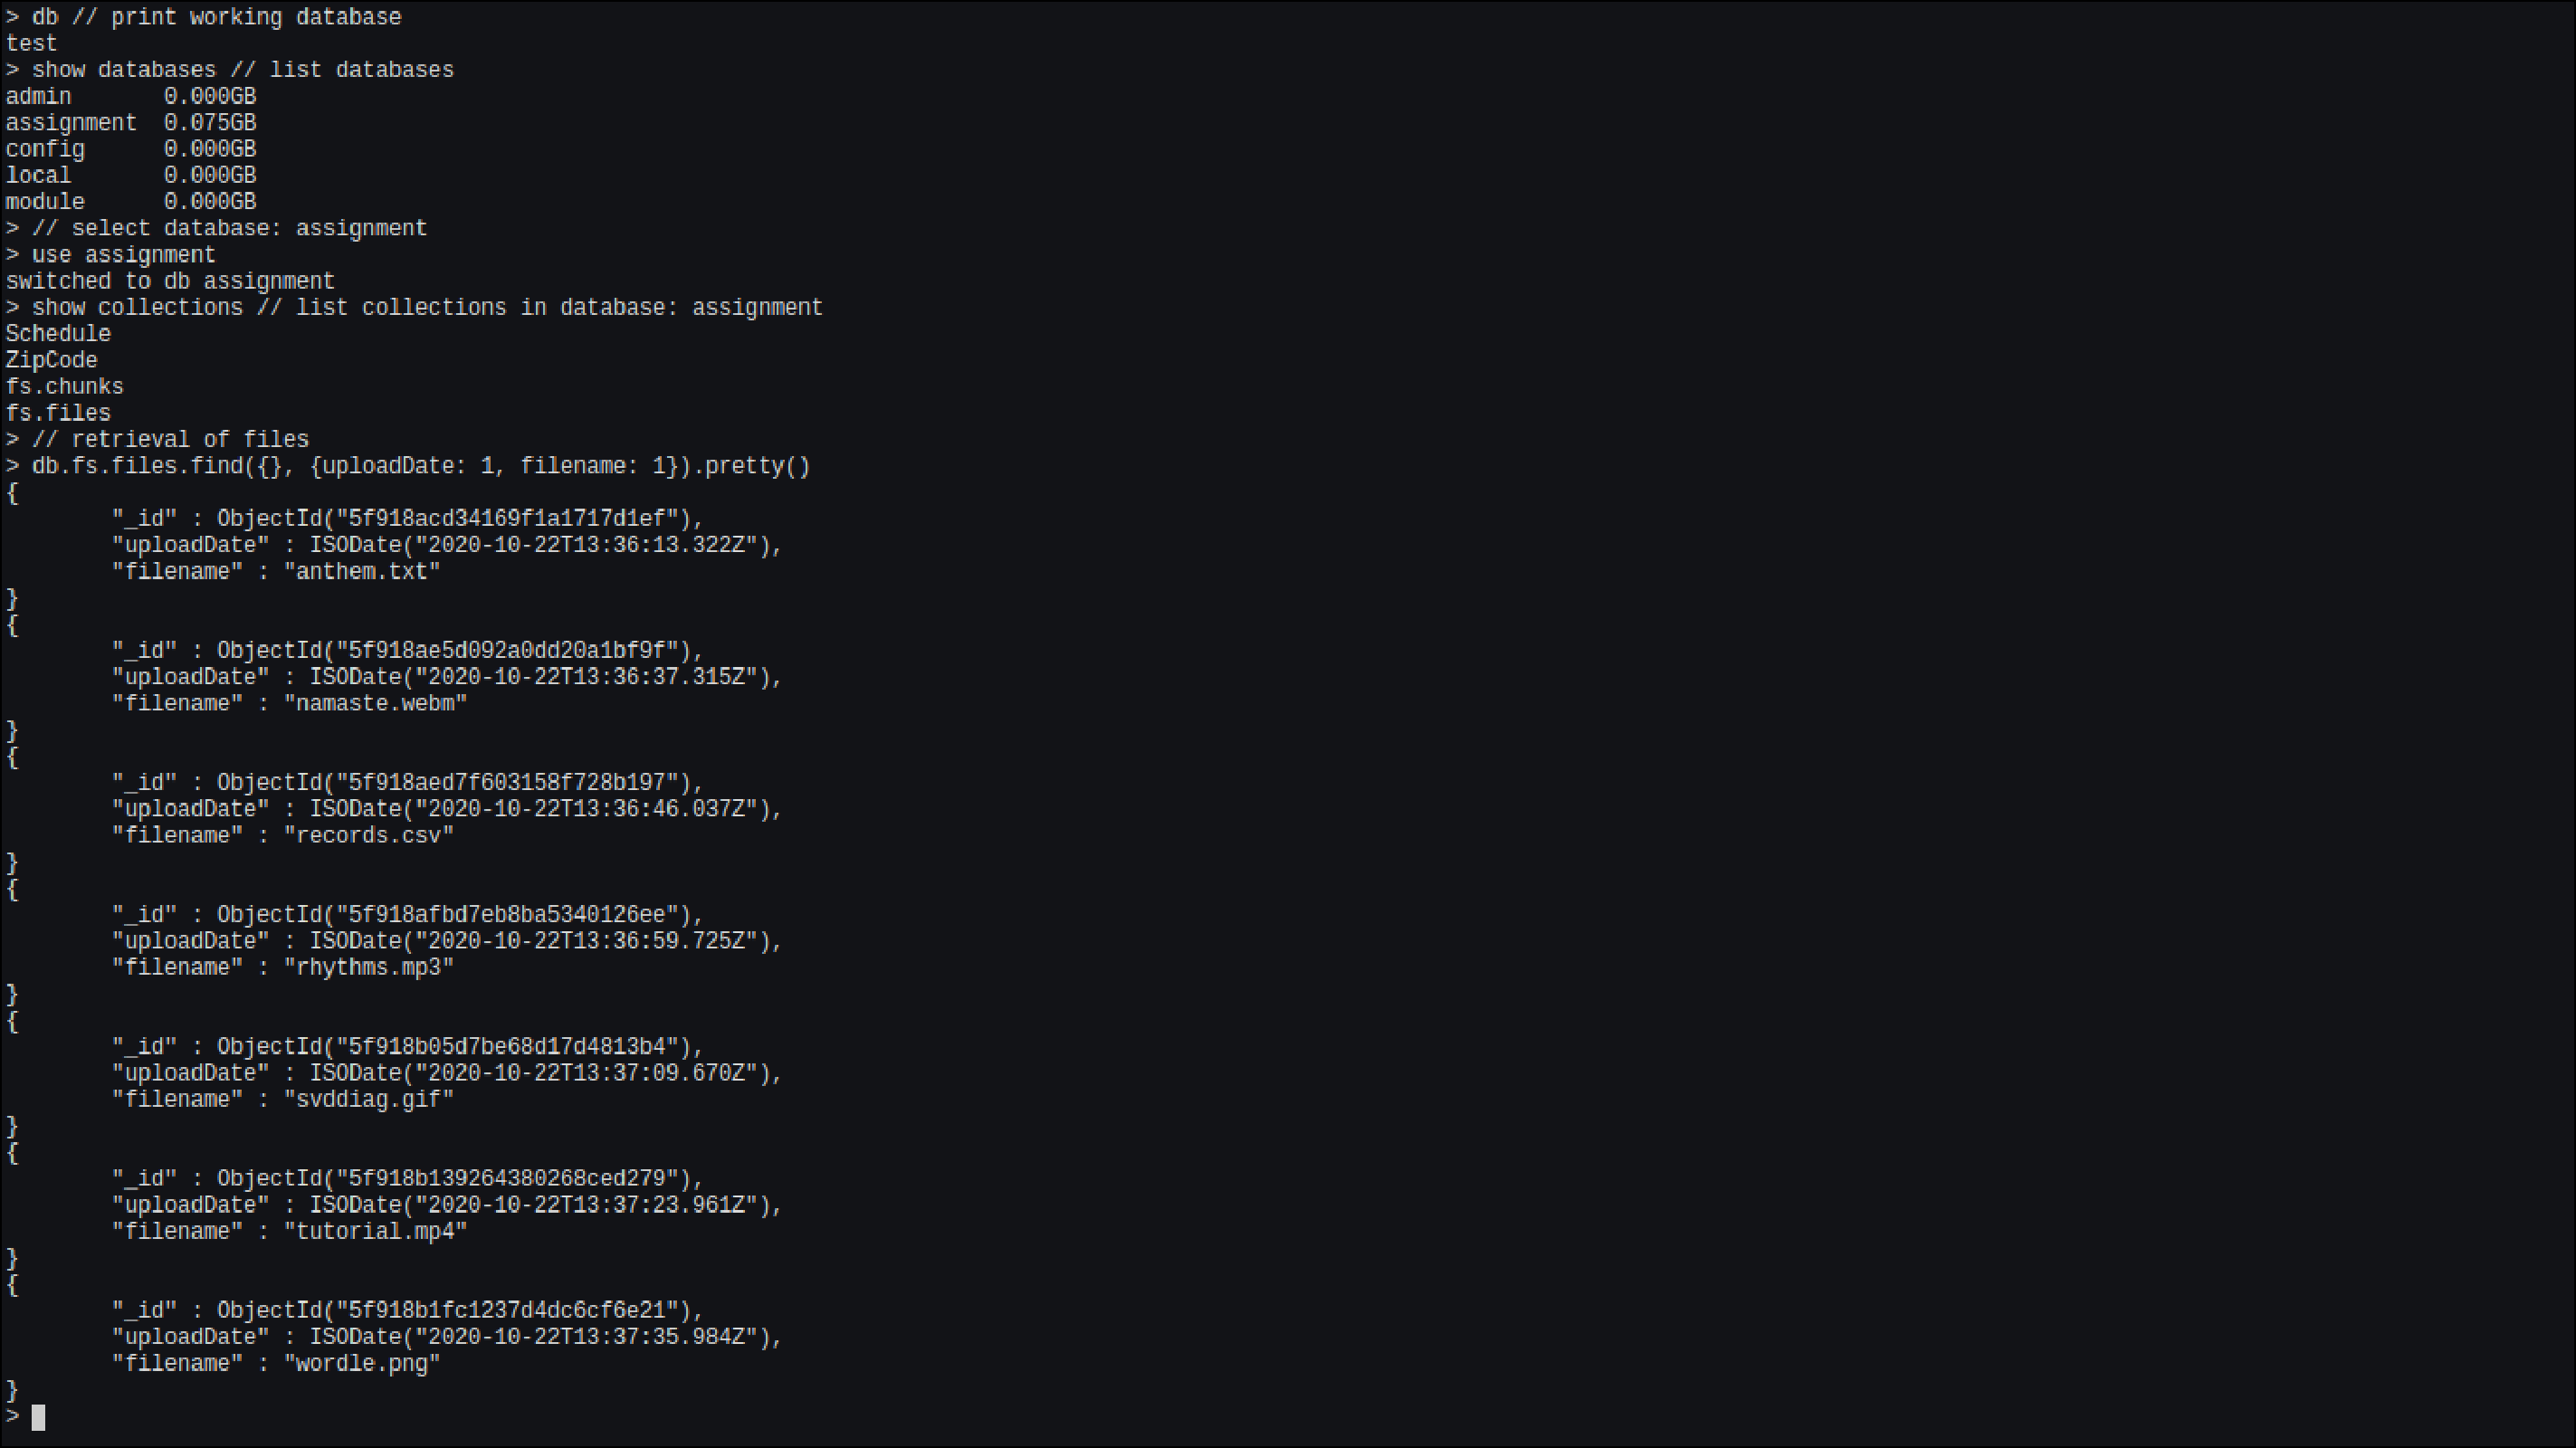
\includegraphics[width=20cm,height=10cm,keepaspectratio]{image3.pdf}
\centering
\end{figure}

\vspace{20px}

{\footnotesize Left Join}

%figure_4
\begin{figure}[ht!]
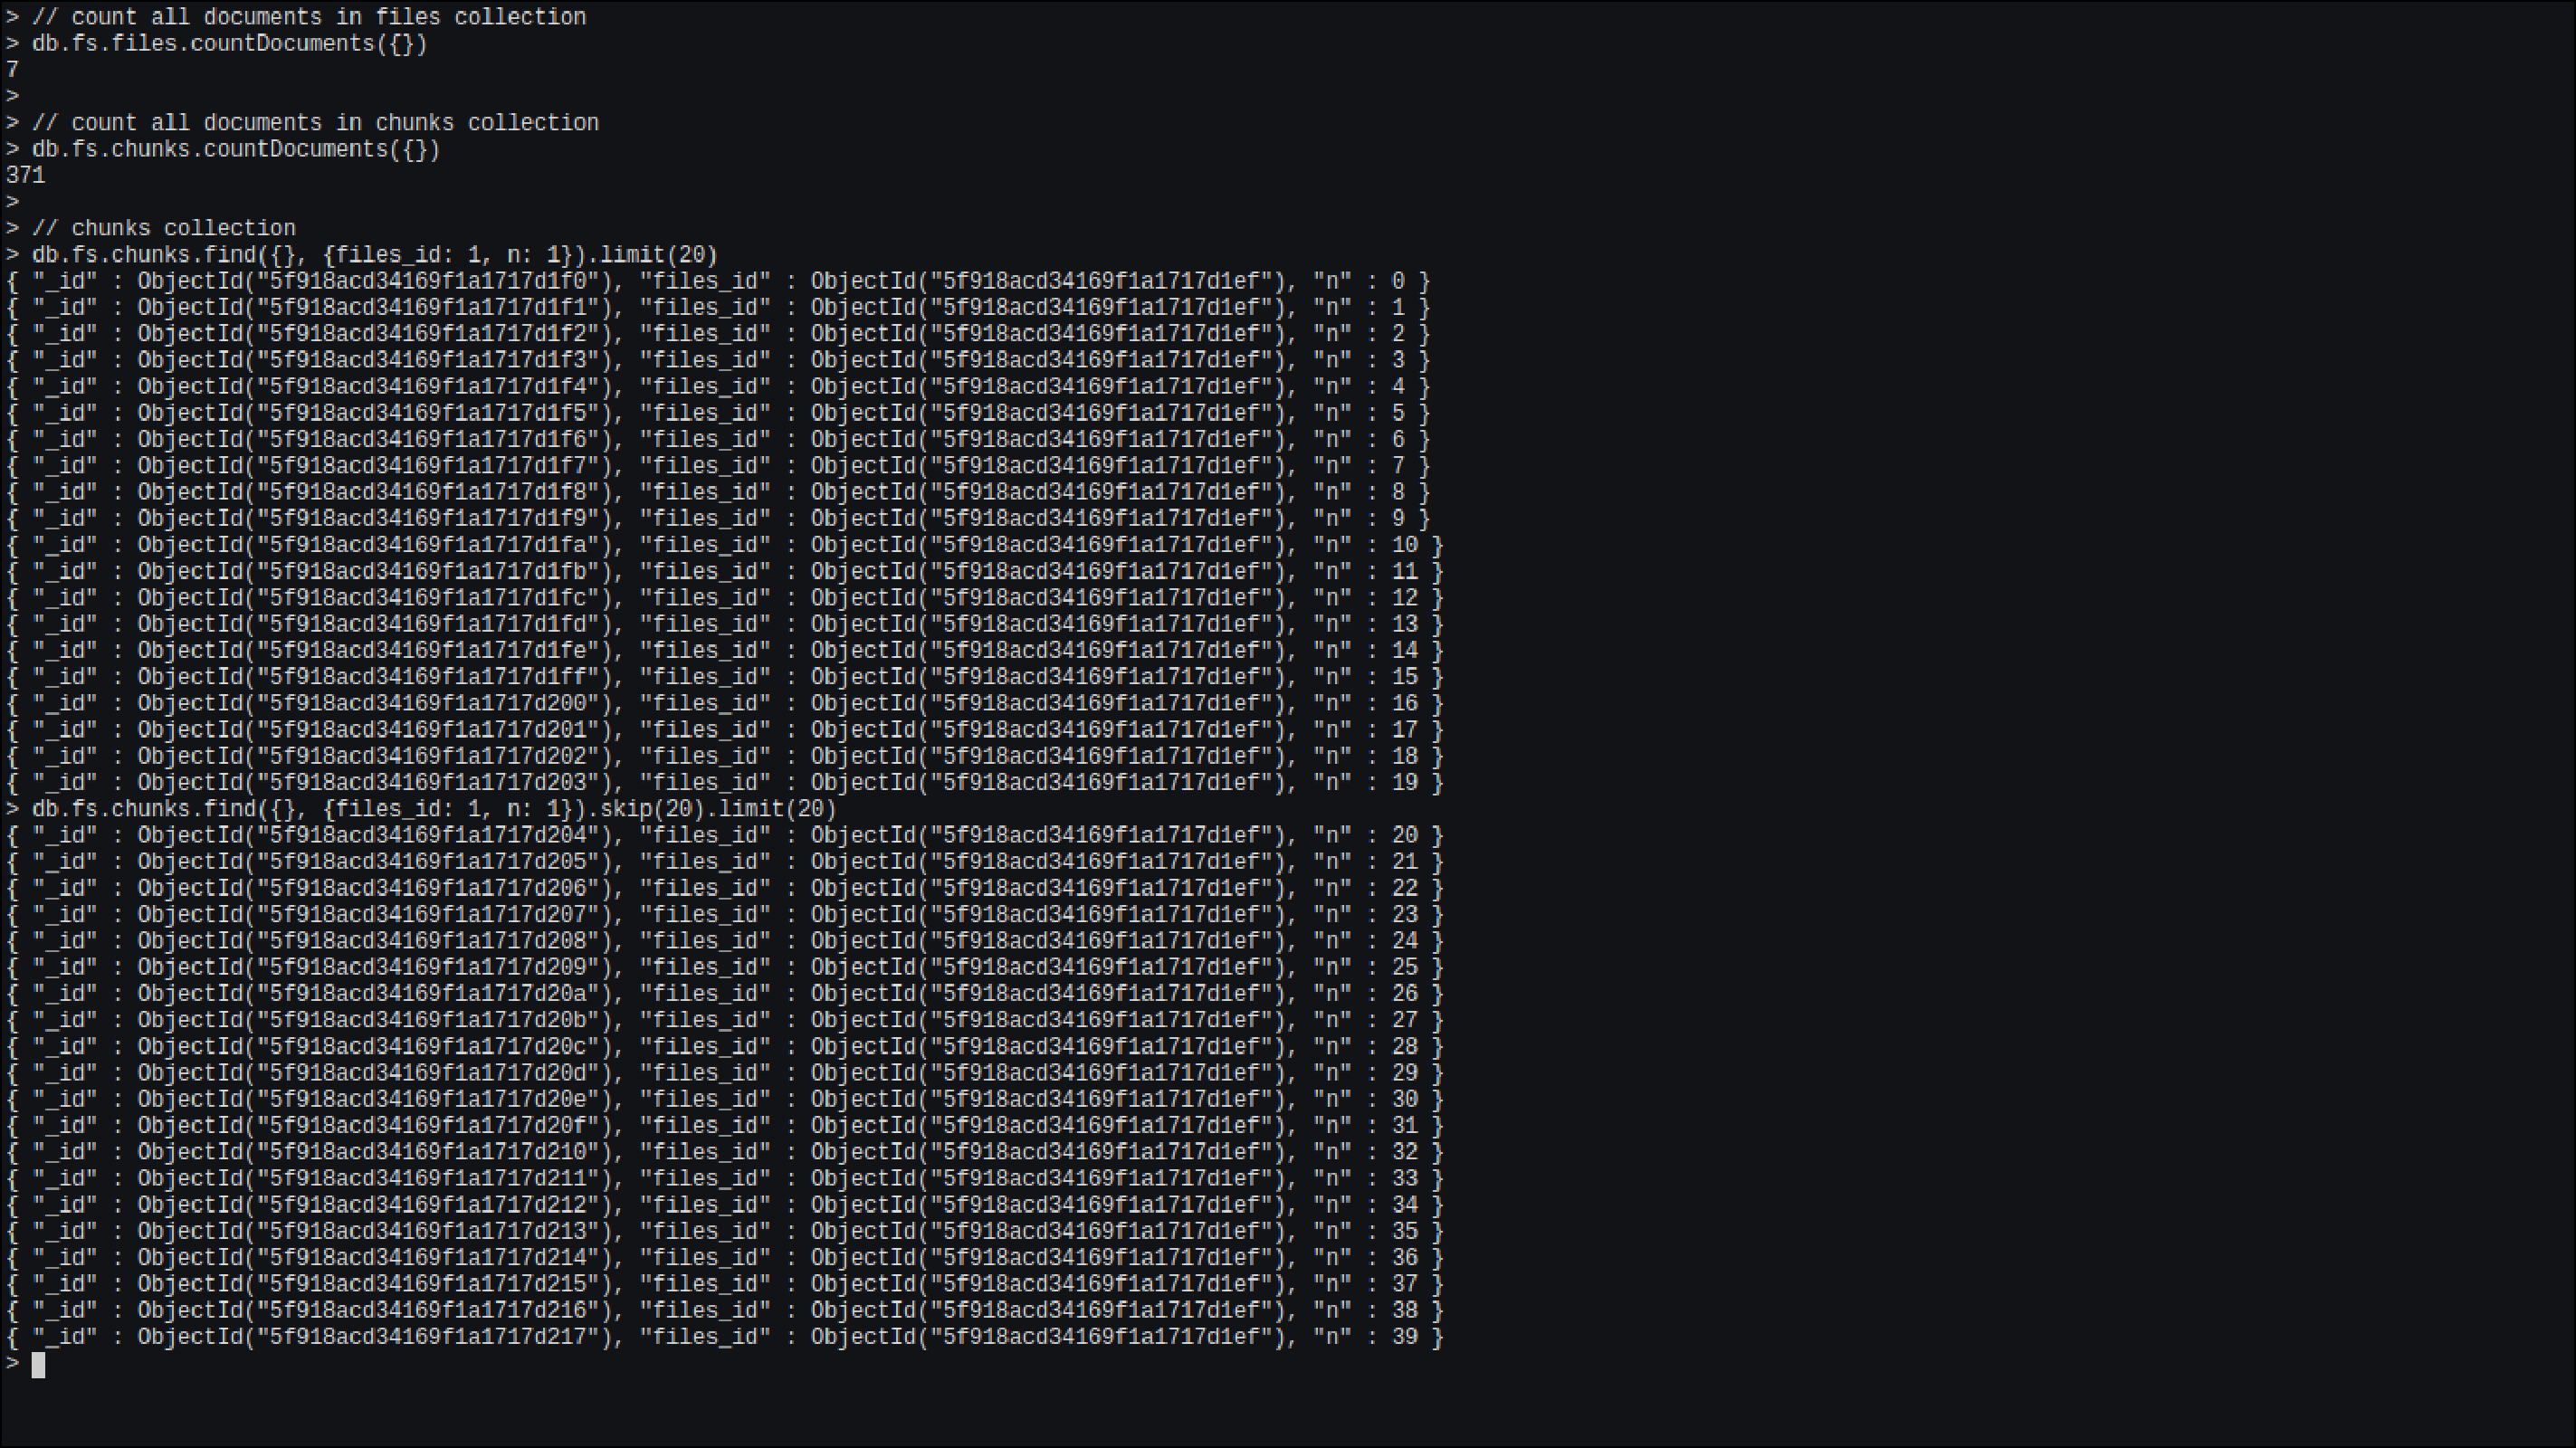
\includegraphics[width=20cm,height=10cm,keepaspectratio]{image4.pdf}
\centering
\end{figure}

\pagebreak

\vspace{20px}

{\footnotesize Right Join}

%figure_5
\begin{figure}[ht!]
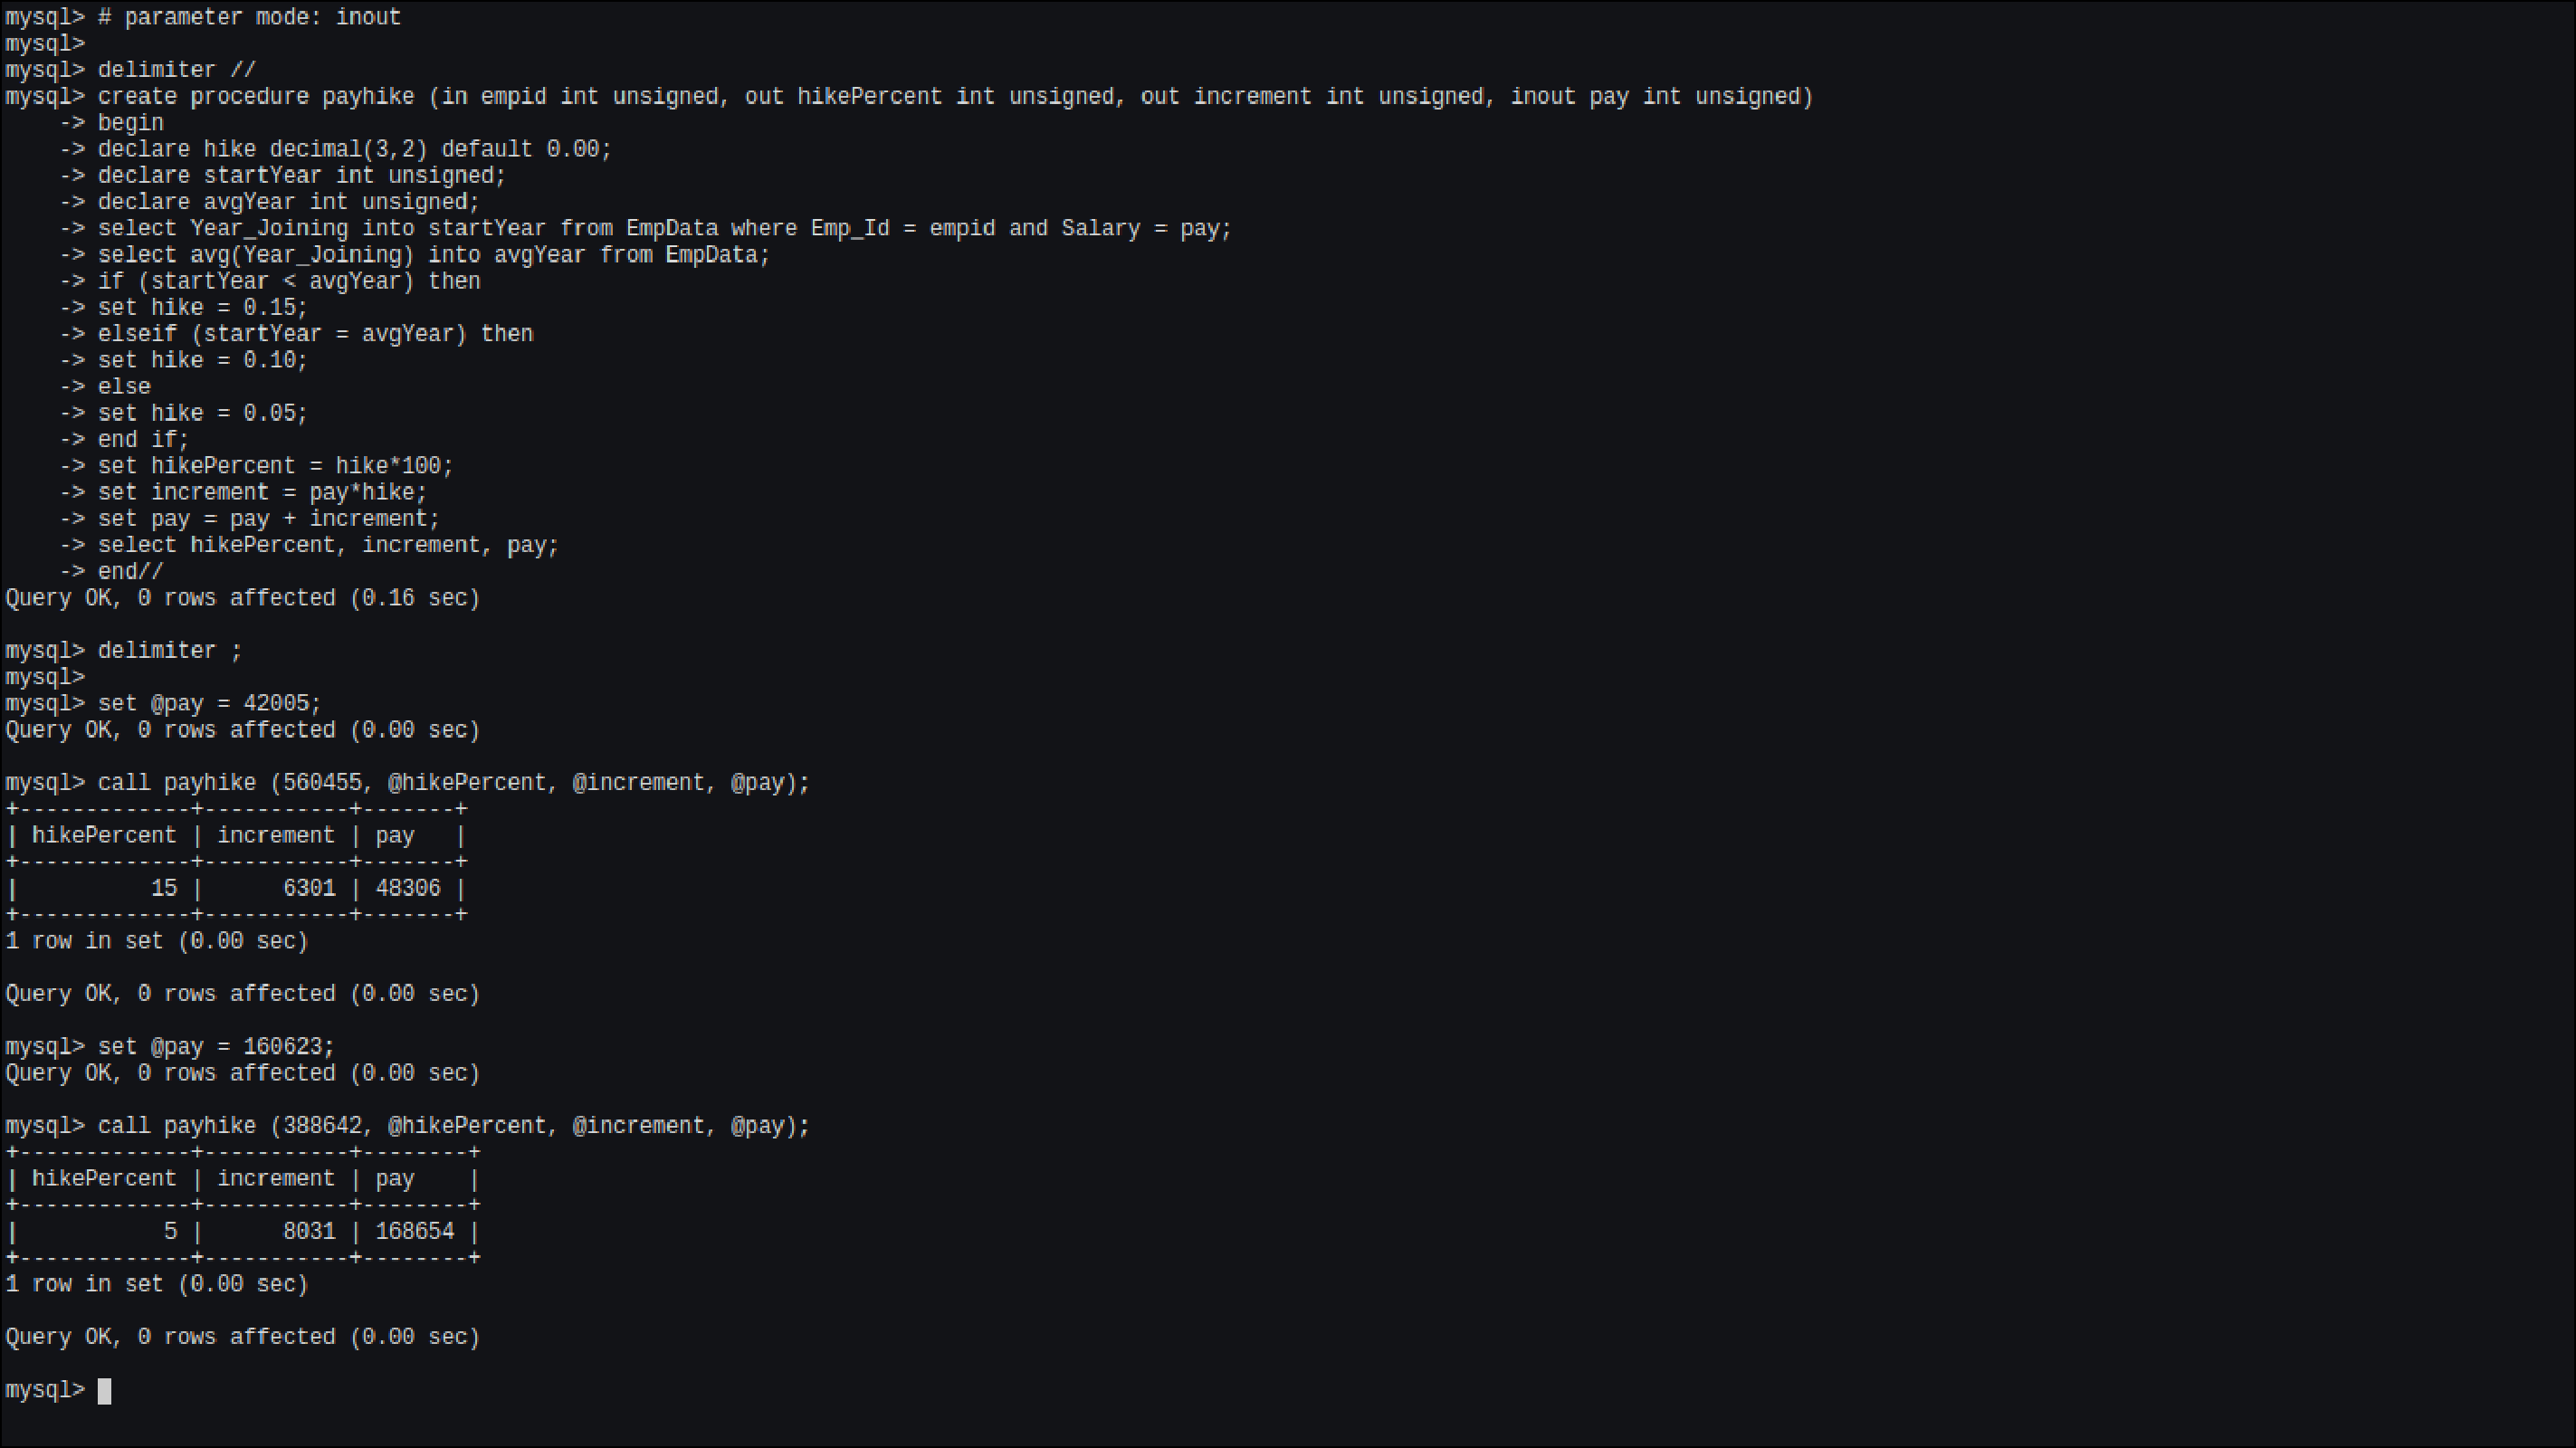
\includegraphics[width=20cm,height=10cm,keepaspectratio]{image5.pdf}
\centering
\end{figure}

\vspace{20px}

{\footnotesize Cross Join}

%figure_6
\begin{figure}[ht!]
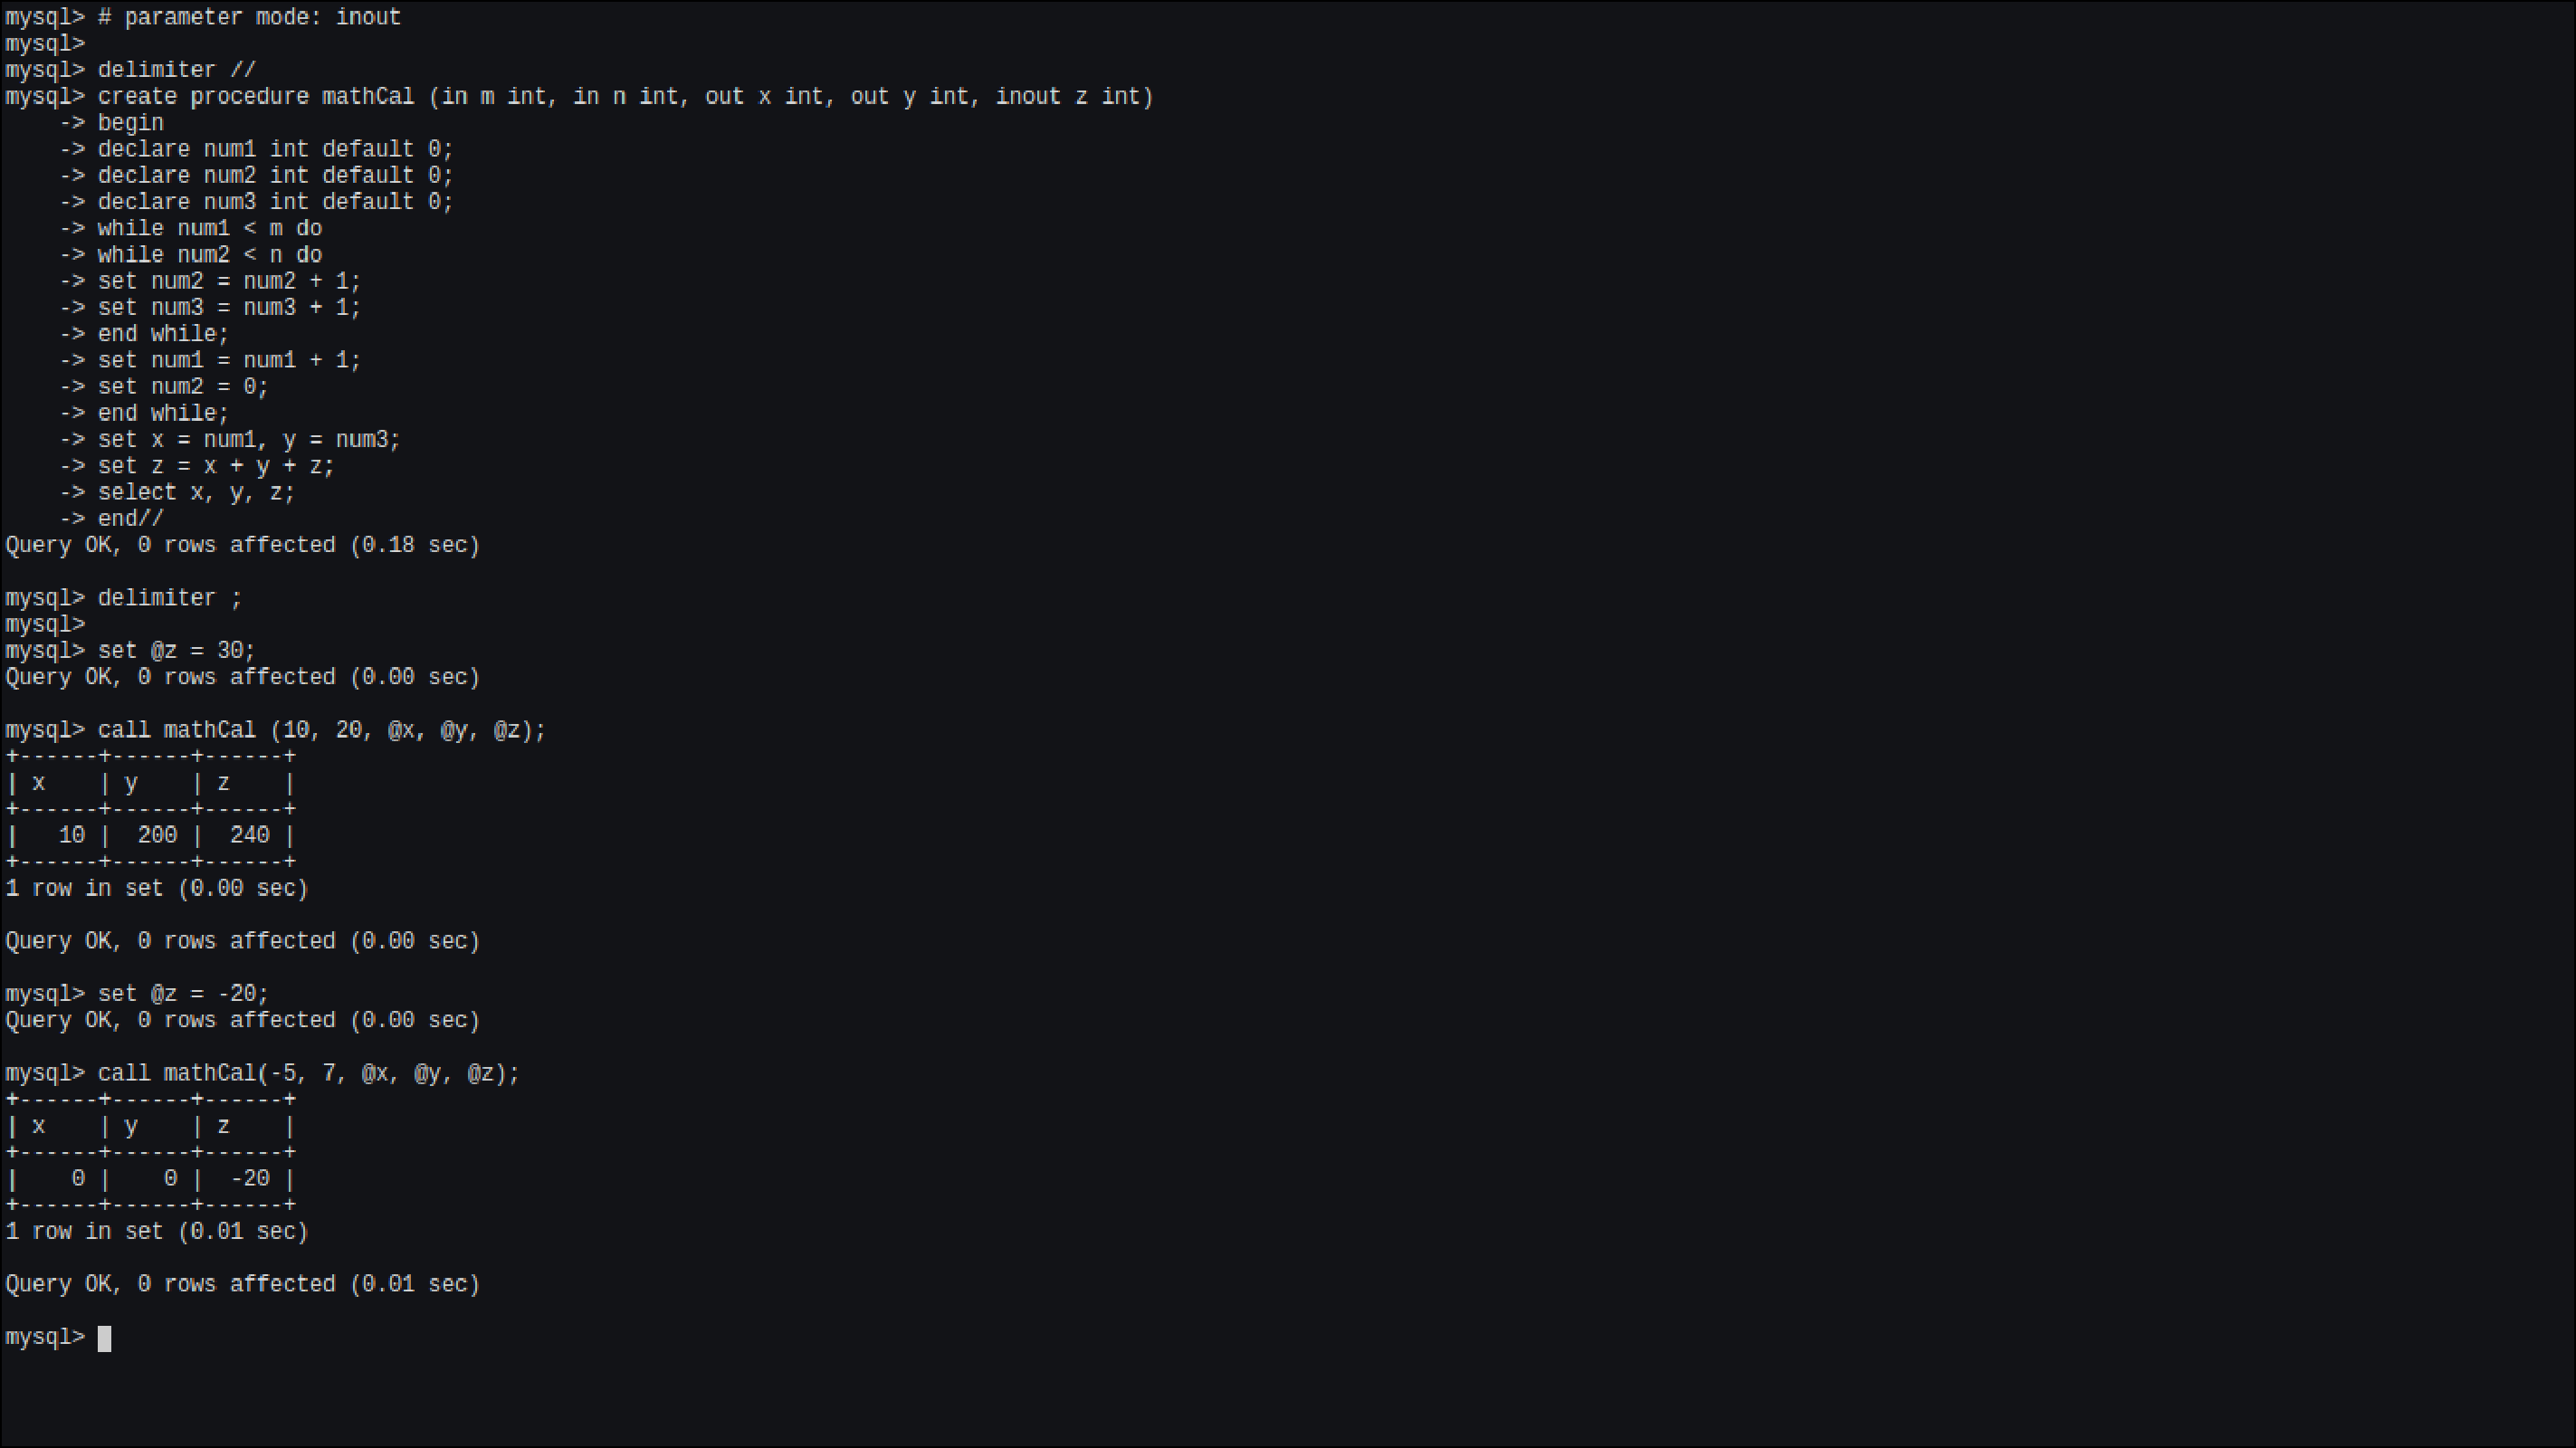
\includegraphics[width=20cm,height=10cm,keepaspectratio]{image6.pdf}
\centering
\end{figure}

\pagebreak

\vspace{20px}

{\footnotesize Group by}

%figure_7
\begin{figure}[ht!]
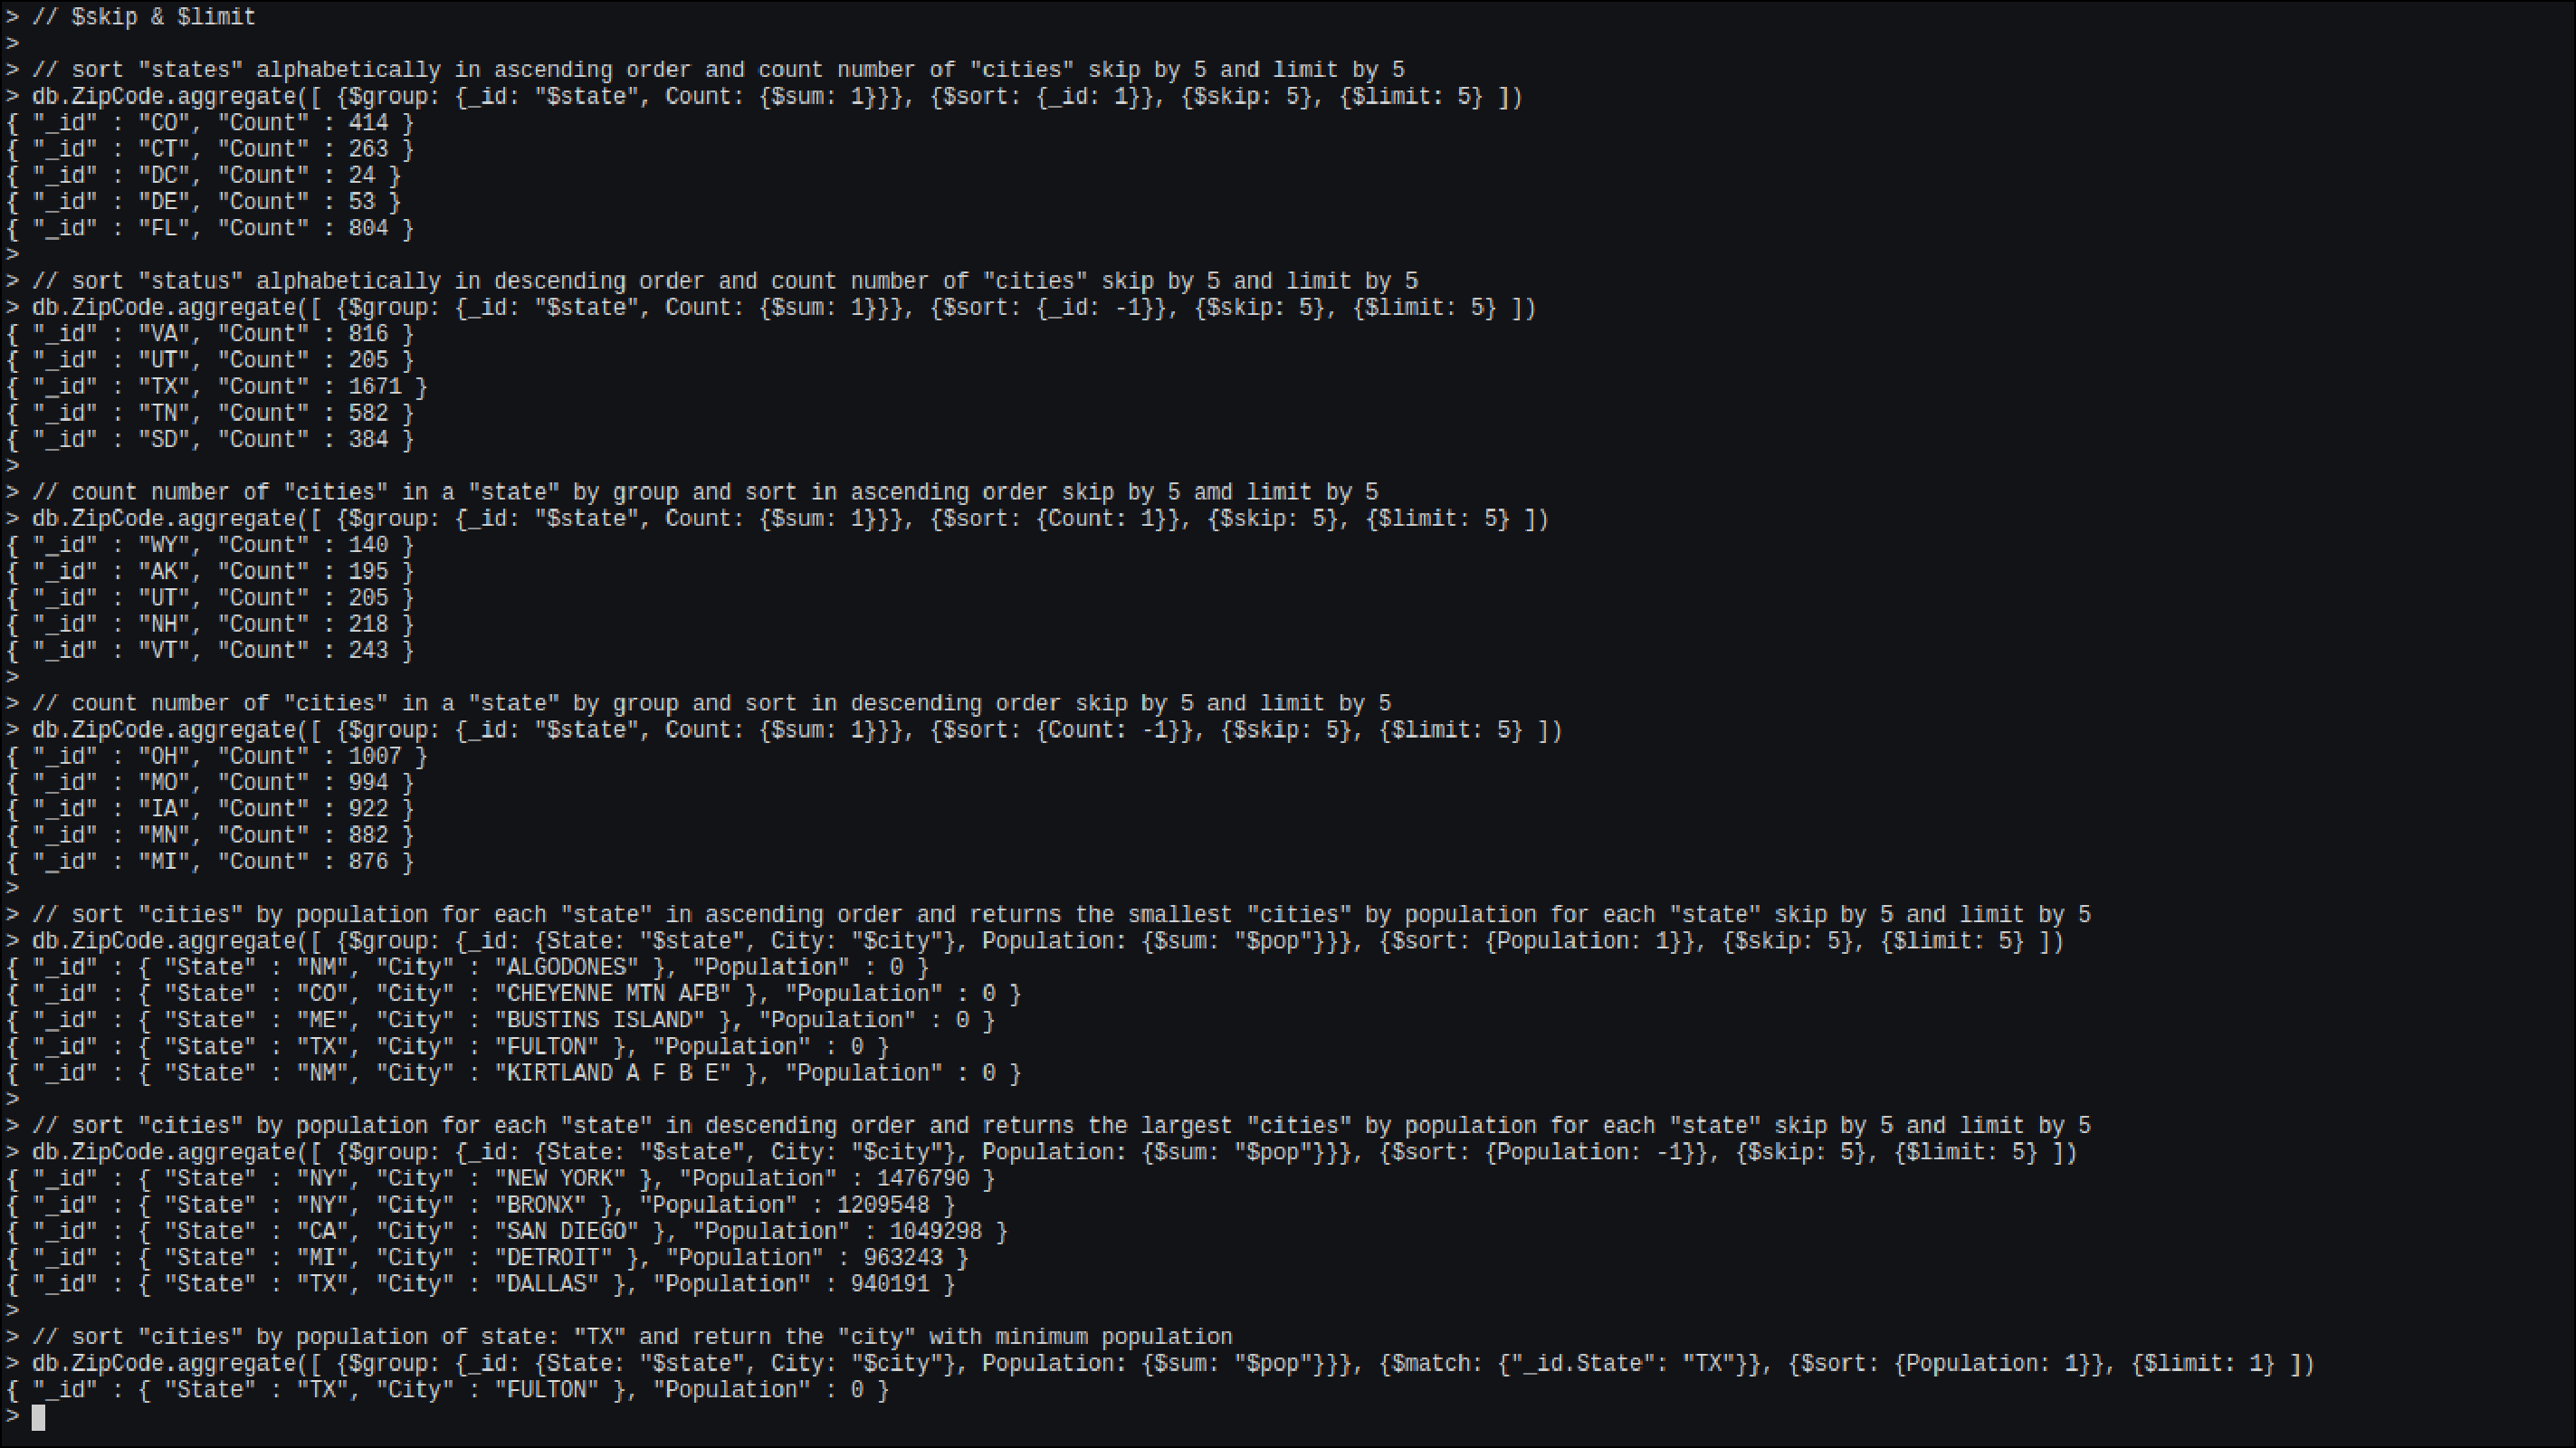
\includegraphics[width=20cm,height=10cm,keepaspectratio]{image7.pdf}
\centering
\end{figure}

\vspace{20px}

{\footnotesize Having clause}

%figure_7
\begin{figure}[ht!]
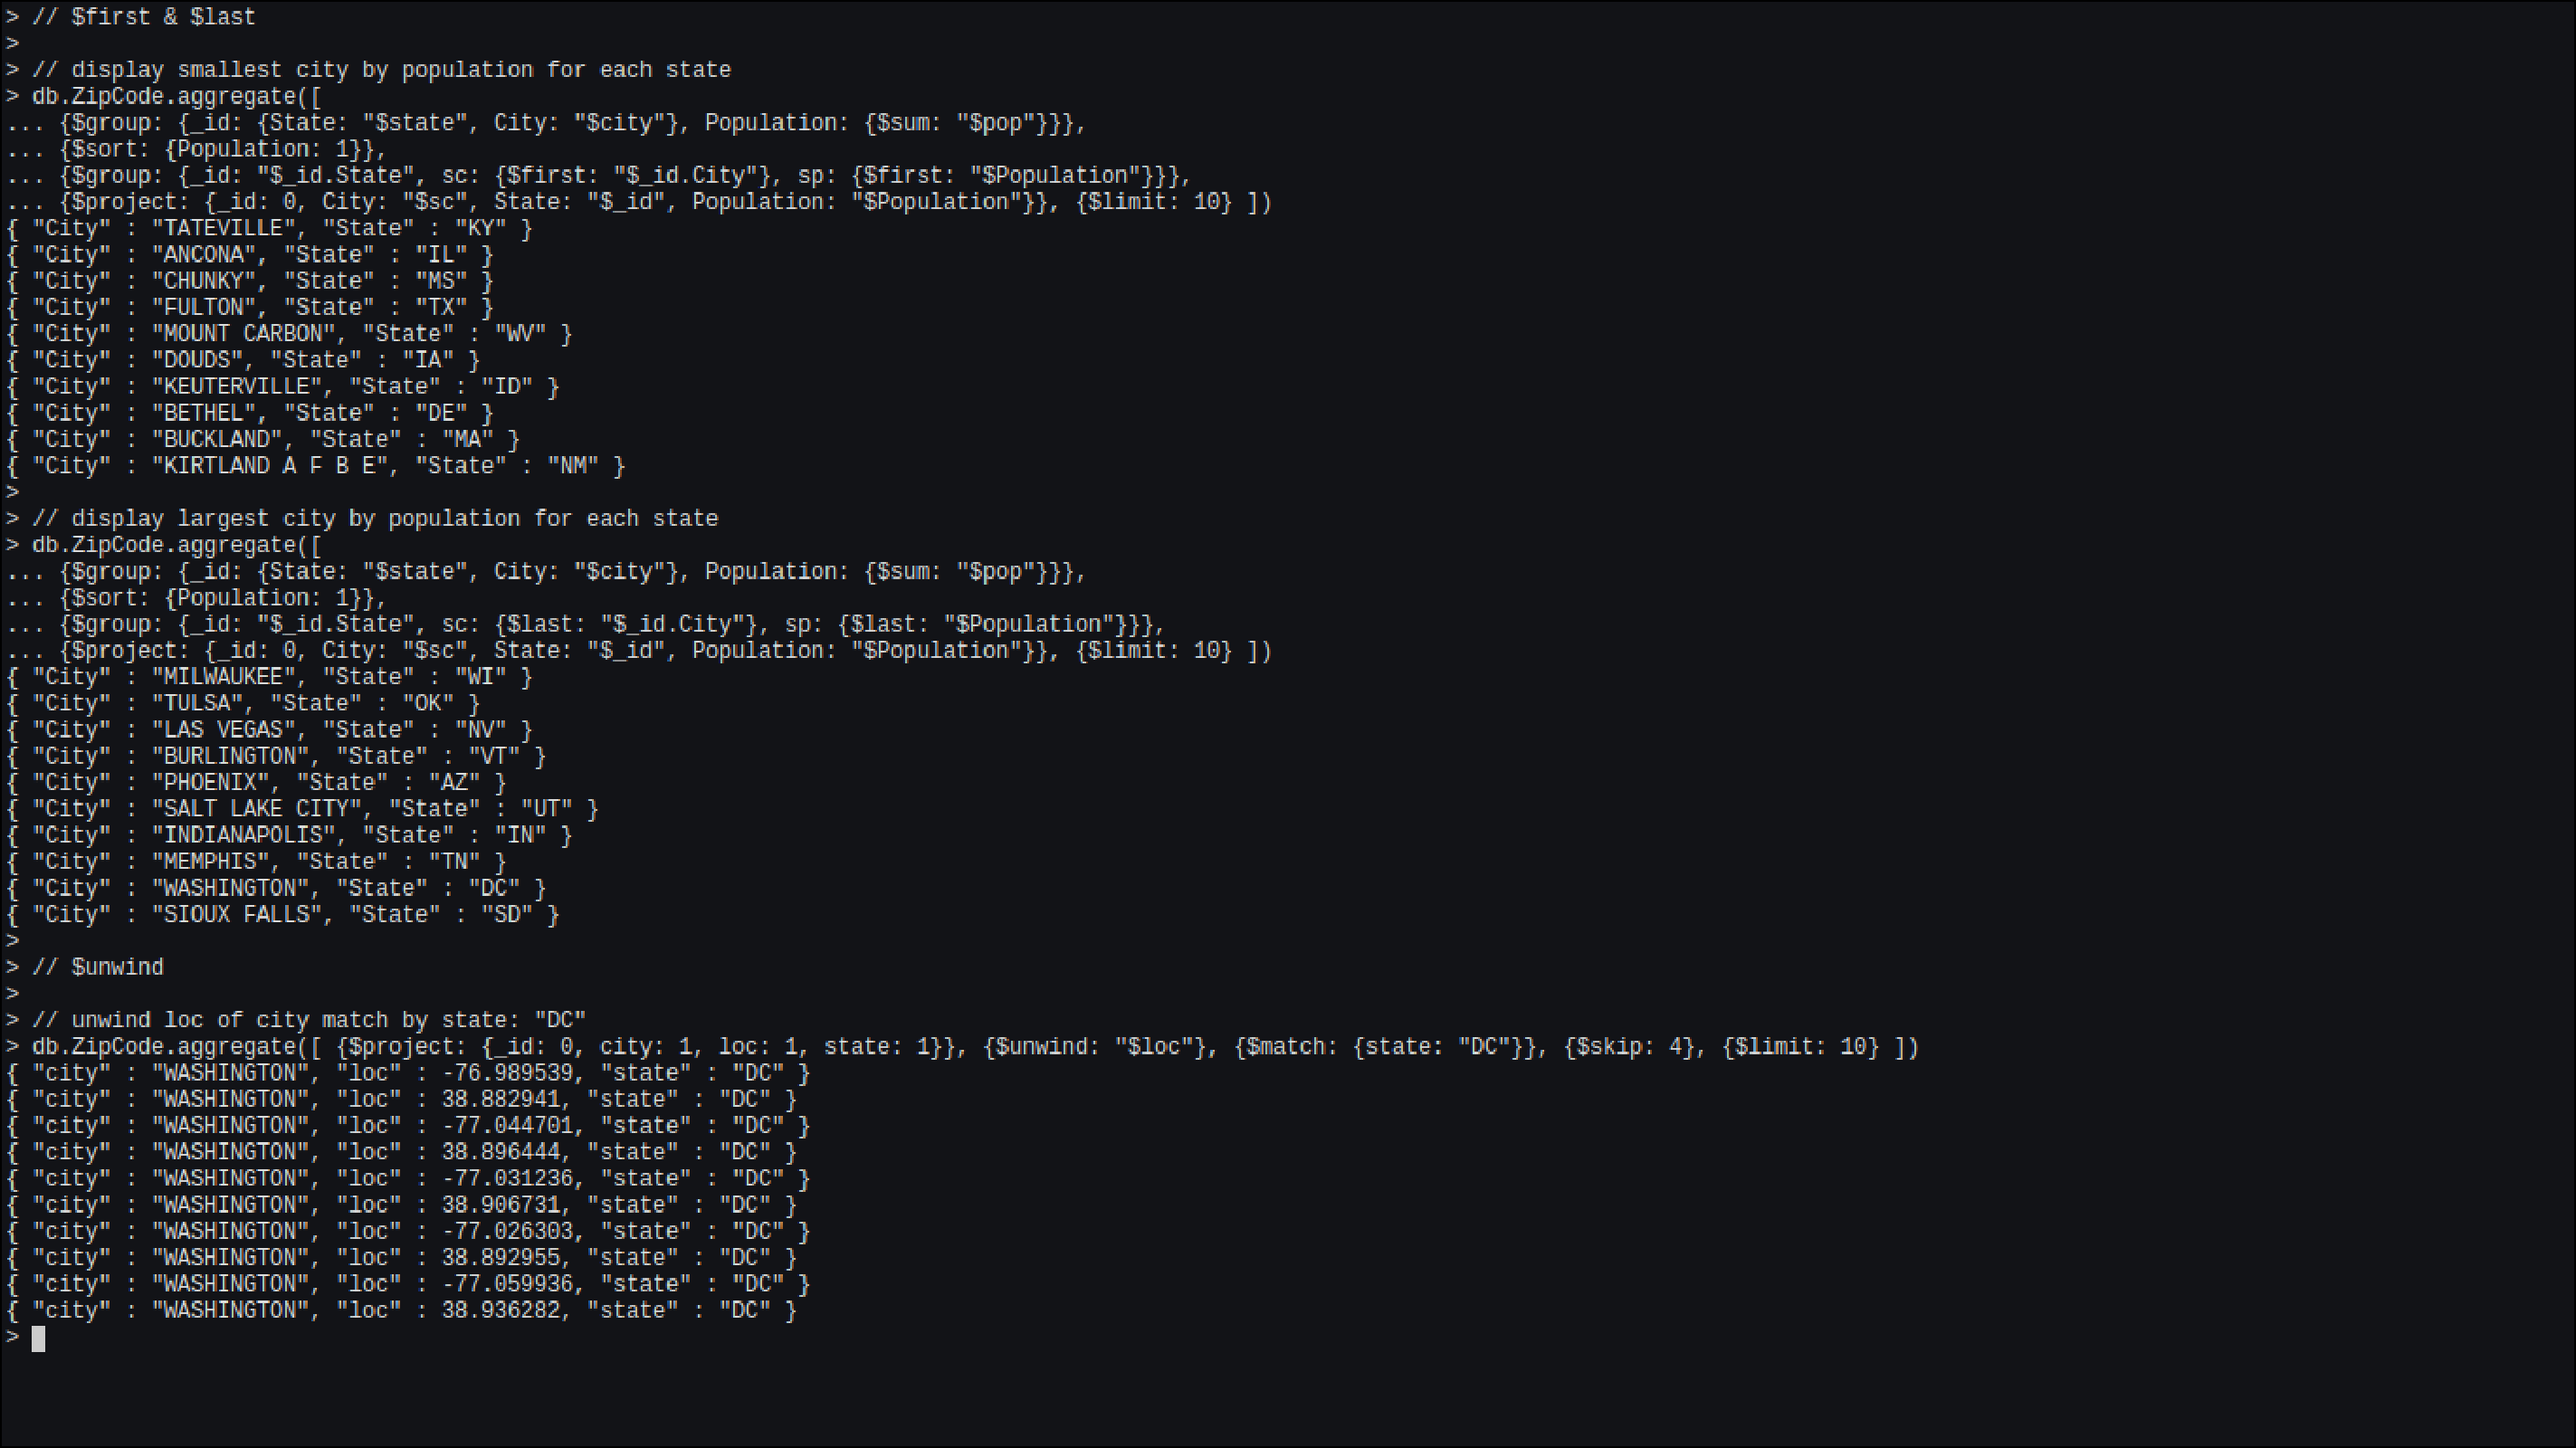
\includegraphics[width=20cm,height=10cm,keepaspectratio]{image8.pdf}
\centering
\end{figure}

\end{document}
